\chapter{Topologies for FPGA-to-FPGA communication}
\label{cha:topologies}

This chapter will describe in detail the topologies which can be setup to
connect the FPGAs using the QSFP ports to perform point-to-point communication
to each other. The first section of the chapter will introduce the possible
topologies which are feasible with the Noctua 32 FPGA system. The second
section will describe the prototypes which were developed to evaluate two
of the topologies to verify the functionality and compare the topologies
in terms of bandwidth capabilities specifically for the MIDG2 application.

\section{Topologies}

As the current available BSP for the Nallatech 520N boards only support serial
point-to-point communication between the FPGAs over direct connections, the
configurations to build a topology is limited by the number of ports which is 
4. The four ports would allow one FPGA to communicate simultaneously with 4
other FPGAs. To extend the communication beyond this, the FPGAs can either
communicate via MPI using the host processor or hop over the FPGAs via the
shortest path. Considering these criterion four topologies are feasible which
either use MPI or hops to extend the communication above the 4 nodes.


\subsection*{Terminologies}

To make the understanding of the topologies clear, this section would introduce
some terms which would be used to describe the topologies in the next sections.
The figure \ref{fig:simple_network} shows a network of two FPGAs.
The FPGAs act as the nodes in this network which are connected to each other
with a direct link. To not confuse with the cluster node which are connected to
each other using 100 Gb/s Intel Omni Path, the thesis will refer
these nodes as FPGA and cluster nodes as node in rest of the text. A network in
which all the nodes are connected to each other with direct FPGA-to-FPGA link
will be called an \textit{Isle}. The communication between isles is either done
using hops or MPI via host. The nodes within the isle can either be fully
connected or partially connected to each other.

\begin{figure}[h]%
    \centering
    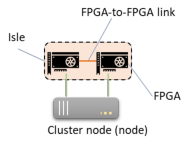
\includegraphics[width=0.6\textwidth]{images/simple_network}
    \caption{Simple network showing the network components}
    \label{fig:simple_network}
\end{figure}


\subsection{Within Node}
\label{sec:within_node}

The simplest topology possible is to connect the FPGAs of a node to each other
using a single channel or all the four channels forming an isle of two nodes as
shown in the figure \ref{fig:within_node}. The FPGAs can only communicate to
each other directly over the channel(s) utilizing the complete bandwidth of the
channels. The topologies can be scaled by adding more isles which communicate
to each other using MPI via the host using the Intel Omni Path. The topology
is simple and easy to setup. Applications which have large amount of data which
needs to be transferred between the processes can benefit from this topology by
efficiently partitioning and distributing the data among the isles and FPGAs.

\begin{figure}[h]%
    \centering
    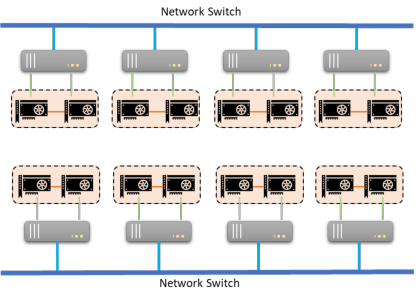
\includegraphics[width=0.8\textwidth]{images/within_node}
    \caption{Within Node topology with two node per isle}
    \label{fig:within_node}
\end{figure}

\subsection{Fully connected}
\label{sec:fully_connect}

The second topology extends the single node topology to two nodes such that
an isle contains four nodes fully connected to each other with separated 
point-to-point link as shown in figure \ref{fig:fully_connect}.
Each FPGA in this topology can communicate with three
other FPGAs simultaneously. Scaling the topology to more nodes can be achieved
in two ways. The first way is similar to within node where the isles communicate
using MPI. In this design, to decrease the overhead of exchanging data via the
MPI, the data should be collected on a single FPGA using the point-to-point
link and then exchanged via MPI. On the receiving end the process can be
reversed. Some more details of possible strategies to scale this design
effectively would be discussed in section \TODO{add reference} 

\begin{figure}[h]%
    \centering
    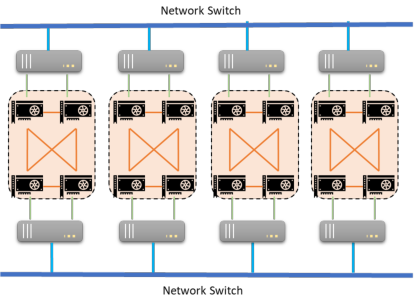
\includegraphics[width=0.8\textwidth]{images/full_connect}
    \caption{Fully connected topology of four FPGAs per isle}
    \label{fig:fully_connect}
\end{figure}

The second way to scale the design is to use the extra link left on the 
FPGAs to connect the isles to each other with two FPGA-to-FPGA links which is described in the section \ref{sec:connected_graph}.

\subsection{Connected Graph}
\label{sec:connected_graph}

This topology is an extension of the fully connected topology of the fully
connected topology. The isle formed by the fully connected FPGAs is connected
to each other using the fourth free port forming a connected graph network
as show in figure \ref{fig:connected_graph}.
In this topology all the FPGAs can communicate to each other without requiring
any data communication via host. In addition to the knowledge of fully
connected mapping within the nodes, additional information about the neighboring
isles would be required to be stored or configured in the FPGAs at compile time
or at runtime. The additional information would be used by the FPGA to create
a mapping table to route packets to the destination FPGAs via the shortest path.
A data to be transferred from one FPGA to another in a different isle would
then have to hop over the FPGAs along the shortest path to reach
from source to destination.

\begin{figure}[h]%
    \centering
    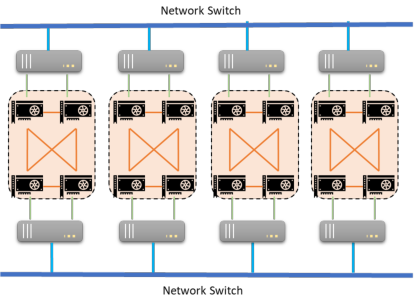
\includegraphics[width=0.8\textwidth]{images/full_connect}
    \caption{Connected Graph with HOPs between fully connected groups}
    \label{fig:connected_graph}
\end{figure}

This thesis proposes this topology as possible scaling design and there was no
implementation and evaluation done for this topology as part of the thesis.

\subsection{Toroidal}
\label{sec:toroidal}

The last feasible topology for the FPGA network is the toroid. As explained by
\textcite{robertazzi_toroidal_1988}, A two dimensional toroidal network is
a network in which the nodes on the left and right boundaries and the
nodes on the top and bottom boundaries are connected to each other giving
a fully connected network. The length and breadth of the network can vary
depending upon the application requirements. As the maximum number of
connection for per node required in the toroidal network is 4, the toroidal
suits a lot to create a fully connected network of the FPGAs.

As Noctua has 32 FPGAs, two 4 X 4 torus as shown in figure \TODO{Add torous
network} would be appropriate for connecting the FPGA giving an equidistant
hops in each direction. The actual routing and packet forwarding strategies
were not investigated in this thesis due to higher complexities
and lack of hardware resources to achieve a result as part of the thesis.

\begin{figure}[h]%
    \centering
    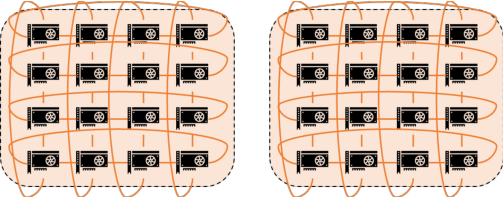
\includegraphics[width=1.0\textwidth]{images/torus}
    \caption{Two Toroidal network to connect 32 FPGAs}
    \label{fig:toroidal}
\end{figure}

\section{Evaluated Topologies}

This section would describe the prototypes developed to evaluate the topologies
introduced in sections \ref{sec:within_node} and \ref{sec:fully_connect}.

